% !TEX root = ../Masters.tex
\chapter{Introduction}
\label{chap:introduction}

\section{Topic covered by the project}
\label{sec:topic}

This project covers the topic of \glsfirst{EA} which is part of evolutionary computing and even more broadly artificial intelligence.
More specifically, it covers the use of \gls{EA} to evolve \glspl{L-system} into good graphical models of aesthetically pleasing plants.
% which is one form of \gls{PCG}~\cite{PCG_5}.

\glspl{L-system} were originally conceived as a mathematical model for cellular interactions in development~\cite{1968Lindenmayer-1,1968Lindenmayer-2}.
From this, geometric interpretations of L-systems have been created so that they can be used to model plants~\cite{2012Prusinkiewicz}.
An L-system is a rewriting system, meaning that it rewrites itself based on a set of rules defined by a grammar.
A simple example is an L-system with the rules $a \rightarrow b$ and $b \rightarrow ba$, and the axiom $a$.
Based on the rules, the $a$ axiom is first rewritten to $b$.
Then $b$ is rewritten to $ba$, $ba$ is rewritten to $bab$, which is rewritten to $babba$, and so on.

These rewritten strings do not mean anything on their own, and that is where the interpretation comes in.
If we interpret $b$ as rotating 45° left and $a$ as drawing a line 1 cm forward, the L-system would model a growing structure, as visualized in Figure~\ref{fig:example-l}.
If the alphabet is expanded from only $a$ and $b$, and more interpretations are added, L-systems can model complex structures in both 2D and 3D, such as plants.

\begin{figure}
    \centering
    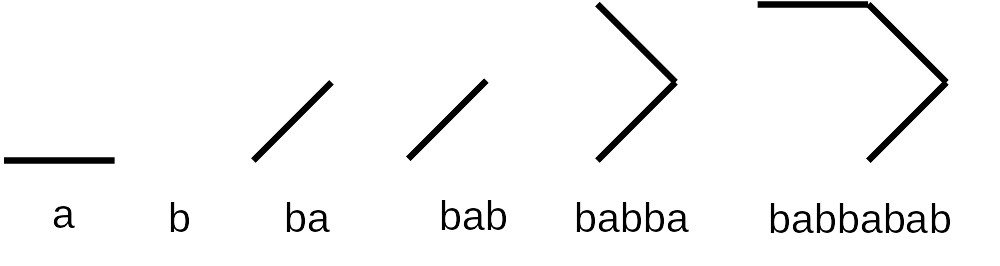
\includegraphics[width=0.8\textwidth]{figures/lsystem}
    \caption{Example L-system being rewritten and interpreted}
    \label{fig:example-l}
\end{figure}

How do you then create L-systems that model the complex structures you desire?
They could be hand crafted by manually defining the rules, but this is difficult for non-experts and require significant amounts of experimentation and analysis of the desired structure~\cite{1993McCormack}.
Additionally, what if an exact structure is not desired, but rather a structure that fulfills some requirement, for example being aesthetically pleasing?
This is where \gls{EA} is useful.

\gls{EA} is not directly connected to L-systems, but it is a tool that can be used to evolve data structures, such as \glspl{L-system}.
\glspl{EA} generate an initial population of structures, then repeatedly evaluate their quality, select structures to reproduce, reproduce them and replaces the population with the new structures until they are satisfied~\cite{2006AshlockEA}.
By repeatedly selecting good individuals and reproducing them, \gls{EA} may find solutions to problems that perform exceptionally well.
It is used in many fields, and has many applications.
For example, \gls{EA} has been used to find weights for an \gls{ANN} that is used in a virtual robot, it has been used to optimize the fuel consumption of stoves, and is being used for modeling complex or noisy data~\cite{2006AshlockEA}.
Finally, it has of course been used to evolve L-systems, both simple fractal structures and 2D and 3D plants~\cite{1998Mock,1998Ochoa,2002Ebner,2003Ebner,2006Ashlock,2009Beaumont,2009Corchado,1994Jacob,2000Vanak,2001Hornby,1995Jacob, 1996Jacob, 1996Jacob-2}.
% used in many fields
% robot, ANN, stoves (Nicaragua), modelling complex or noisy data,

% In the area of computer graphics, visualization and game development, there is a desire to replicate environments and creatures found in nature in a virtual environment. %cite
% Many types of environments and creatures can be of interest, for example terrains, mountains, rivers, plants, animals and bacteria.
% These can be created by manually modeling the specific objects, for example by 3D artists, but this can be a slow process, especially when a large variation of the objects is required.
% Another approach is to generate the content using \gls{PCG} methods.
% This way, digital programs can generate virtually infinite amounts of variations based on a representation and a recipe.

% Plants, specifically, can be generated using \glspl{L-system} where their structure is represented as strings of characters in a parallel rewrite system~\cite{2012Prusinkiewicz}.
% Based on actual plants, one may model a virtual plant by creating the rewrite rules and parameters for how the system should be drawn.
% These models can be handcrafted, or alternatively \gls{EA} can be applied to evolve the models into something desired.

\section{Keywords}
\begin{itemize}
    \item L-system
    \item plants
    \item artificial intelligence
    \item evolutionary algorithm
    \item genetic algorithm
    \item grammatical evolution
    \item procedural content generation
\end{itemize}

\section{Problem description}
\label{sec:problem}
Real plants can be bred to create offspring with desirable features from multiple species.
For example, many of the species used in agriculture have gone through selection over several years to yield plants that produce a bigger quantity of food and are resistant to diseases and harsh environments.
Some plants were domesticated several thousand years ago, for example the popular plant Maize has indication that it was domesticated 8700 years ago~\cite{2009Starch}, while crossing between different species started in the 18th century~\cite{PlantBreeding}.
This can be a complex and long process, taking several hundreds of years with gradual improvements, and many combinations do not even work.~\cite{2014Hartung, PlantBreeding}

To make this process more fun and interesting, a virtual world where people can breed plants could be created.
In this world, breeding is not limited like it is in the real world.
Plants could be combined in ways never thought to be possible.
For example, a user may like both apple trees and Venus flytraps, so they want to combine them into a tree with Venus flytrap mouths of a size that could eat humans.
The problem is that randomly crossing the representation of different plants may not produce meaningful or interesting offspring, but rather random creatures that do not satisfy the user.

To be able to create meaningful crossovers between virtual plants, a baseline requirement is to have something that models the plants and something that generates the plants.
The plant model is a baseline requirement of the system, as no generator or crossover would work without this, and a generator is required to generate the parent plants.
Additionally the generator could be used to cross the plants into something the user is satisfied with.

Plants that are to be bred should be varied in their shape and features, like real plants are, otherwise interesting combinations can not be made.
Additionally, since the breeding should be able to create combinations that are impossible in the real world, the variation should be even larger, allowing for plants not found in nature.
As a baseline the plants should be aesthetically pleasing, otherwise the user of a virtual environment with these plants would most likely be dissatisfied.
This is especially important in video games where a user may quit if they do not enjoy playing it.
Finally, if the plants should be crossed, their model should be represented in such a way that genes can be interchanged in a meaningful way that retains the properties of the plants.

The current research on evolving \glspl{L-system} using \gls{EA} uses strict restrictions on the grammar which limits the variation in the plant, in addition to its potential for being aesthetically pleasing. %cite...???
Thus a less restricting grammar is required, but this will increase the complexity of the problem, making it more difficult to produce meaningful and pleasing plants.

In summary the problem to be studied is how to generate aesthetically pleasing and varied \gls{L-system} plants that could be used for crossbreeding, with a particular focus on how to handle complex grammars.

\section{Justification, motivation and benefit}
As is apparent from Chapter~\ref{chap:background}, currently \gls{EA} has only been applied to restricted L-systems or only parts of L-systems.
The research often only studies the simplest types of L-systems~\cite{1998Mock,1998Ochoa,2002Ebner,2003Ebner,2006Ashlock,2009Beaumont,2009Corchado}, while sometimes also the more versatile parametric L-systems~\cite{1994Jacob,2000Vanak,2001Hornby}.
In both cases, the L-systems are usually based on assumptions about the size of the alphabet, string lengths, number of productions and branching depths.
This restricts the potential power of L-systems, thus also restricting the potential of generating complex and intricate structures, for example aesthetically pleasing and varied plants.
This project explores a more expressive L-system as well as techniques to guide the generation of good solutions with it.
While we do not explore the most flexible forms of L-systems, the techniques explored can potentially be applied to these as well.

These benefits are not limited to only \glspl{L-system}, but can be applied to any problems that use \gls{EA} and grammars, for example computer programs, with some modifications.
Looking at the wide specter of applications of \gls{EA}~\cite{2006AshlockEA}, it is apparent that an improvement in \gls{EA} techniques will have indirect beneficial effects for humanity.

Because \glspl{L-system} are used in \gls{PCG}~\cite{PCG_5}, computer graphics, video games and film can benefit from this project.
\Gls{PCG} is defined as ``the algorithmic creation of game content with limited or indirect user input''~\cite{2011Togelius}, and has been used in video games since the 1980s~\cite{PCG_1}.
It can remove the need for artists to lower costs, it may support the artists such that they may be more efficient and create better quality content, it can enable the creation of completely new games, it can adapt the content to the user's abilities or needs, it may allow for more creative solutions than what humans are able to create, and it may help understand design~\cite{PCG_1}.

\Glspl{L-system} and formal grammars in general can be used to generate game content such as plants, missions, spaces and levels~\cite{PCG_5}.
By studying how \glspl{L-system} with \gls{EA} can be used to generate both aesthetically pleasing and varied plants, we will get a better understanding of what factors are important in aesthetic plants, how a wide specter of different L-systems can be generated and how to handle complex spaces in a more efficient manner.
Therefore, this project can improve the techniques used in \gls{PCG} to help the game, graphics and film industries in creating better content and in the end create better experiences for consumers.

With an understanding of how to measure to what degree an L-system plant is aesthetically pleasing, an understanding on how L-systems can be genetically represented and combined, and an understanding of how to generate L-systems in a large parameter space, a basis for combining L-system plants into good offspring is created.
This can be directly useful for \gls{PCG}, as new game concepts or game mechanics of interactions with plants can be created.
Taking this a step further, the findings could be adapted to other types of content, such as game levels where two levels with different concepts should be combined into a new level that borrows concepts from both or combines the concepts into new ones.
In an even broader scope, because \gls{EA} is being used, the techniques may be adapted to other problems, such as \gls{ANN}, computer programs or architecture to search complex spaces or combine two solutions with some desired properties each into one solution with the properties combined.

% The results from this research can be used in a game where users may create their own virtual garden, potentially in virtual reality (VR), where they breed the plants they always wanted to see or new surprising species, and have a place outside the busy world to relax and watch their plants grow.

% The stakeholders in this project are mainly game programmers, game artists, level designers and game developers as a whole.
% Additionally, movie makers and creators of other virtual worlds, like simulators and training software, are included.
% Indirectly game players or consumers in general will also be stakeholders as they consume the content created by the creators.
% At a broader level, stakeholders include \gls{EA} researchers and any field that use \gls{EA}, which is now found in most scientific and non-scientific fields and industries. %cite?

\section{Research questions}
The problem described can be summarized in a single research question: How can we generate \gls{L-system} plants that are aesthetically pleasing, varied and could be used to create offspring similar to its parents?
The base problem to be solved in this question is how to generate plants, and is accompanied with three requirements: being aesthetically pleasing, varied and usable for cross-breeding.
Thus the research question is split into three sub-questions that aim to tackle the three requirements, such that the main research question may be answered.
The questions are listed below.

% The L-systems should be able to represent plants both found in nature and not found in nature, as the problem involves combining existing plants into new plants.
% Thus a new research question is defined: What types of L-systems are appropriate to represent plants both found in nature and not found in nature?
% To combine the L-systems together into offspring with distinct features from both parents, features in an L-systems that appropriately reflect the features found in the produced plants need to be identified.
% This gives raise to the question: What are the features of an L-system that can be combined?
% Finally, the combination of the features needs to happen, and thus comes the question: How can the features be combined to create offspring that contain distinct features from both parents?

\begin{description}
    \item[RQ0] How can we generate \glspl{L-system} plants that are aesthetically pleasing, varied and could be used to create offspring similar to its parents?
    \begin{description}
        \item[RQ1] What \glspl{L-system} models are appropriate to represent plants both found in nature and not found in nature, and that could be combined into new plants?
        \item[RQ2] How can aesthetically pleasing \glspl{L-system} plants be generated?
        \item[RQ3] How can varied \glspl{L-system} plants be generated?
    \end{description}
\end{description}

\section{Contribution}
\begin{itemize}
    \item A literature review of plant \gls{L-system} representations and evolutionary algorithms used on them.
    \item A method of generating well-performing plants from a large parameter space.
    \item An analysis of metrics that evaluate how aesthetically pleasing an \gls{L-system} plant is, and important factors as indicated by humans.
\end{itemize}
